\documentclass[UTF8,a4paper]{ctexart}

%页面边距
\usepackage{geometry}
\geometry{a4paper,left=2cm,right=2cm,top=1.5cm,bottom=1.5cm}

%底部对齐
%\usepackage{balance}
%\balance
\usepackage{flushend}

%在multicols环境中使用figure环境,使用[H]参数
\usepackage{float}

\usepackage[justification=centering]{caption}

%设置页码
\pagenumbering{arabic}
\pagestyle{plain}

%分栏
\usepackage{multicol}

%引入了一些改进的数学环境,如align
\usepackage{amsmath}

%得到引用的标题内容
\usepackage{nameref}

%照片
\usepackage{graphicx}

%添加首行缩进,两个字符
\usepackage{indentfirst}
\setlength{\parindent}{2em}

%多行公式一个编号
\usepackage{amsmath}

%文献引用,标准类型为plain
% \usepackage[hyperref=true,backend=biber,sorting=none,backref=true]{biblatex}
% \addbibresource{article.bib}
\usepackage{cite}

%超链接
\usepackage[linkcolor=yellow,citecolor=red,backref=page]{hyperref}
\hypersetup{
bookmarks=true,
colorlinks=true,
linkcolor=blue
}

%脚注
\usepackage{lipsum}

\title{初探数字图像处理与傅里叶变换}

\author{姓名:寇一笑 \protect\newline
\and 学号:18020024016 \\
\and 专业:电子信息科学与技术}



\begin{document}
\maketitle
\newcommand\blfootnote[1]{%
	\begingroup
	\renewcommand\thefootnote{}\footnote{#1}%
	\addtocounter{footnote}{-1}%
	\endgroup
}%footnote的设置
%\begin{multicols}{2}
\begin{abstract}
	本文主要讨论了傅里叶变换和图像处理\footnote{产生这个想法主要是因为电子专业在大三需要分方向,所以看了一些图像处理方向大三学长的实验报告,里面刚好有提到傅里叶变换,所以读了相关的书籍。学长的报告地址请见$https://github.com/chenfeng123456/CourseInOUC/tree/master/Digital_Image_Processing/report$}的关系。在下面其实只讨论了傅里叶变换和频率域滤波的联系,但实际上图像可以视为一个二维的“滤波”,所以相对应的是一个二维的傅里叶变换,一定程度上用傅里叶变换和频率域滤波的联系也能反映与数字图像处理的关系了。
\end{abstract}

\section{傅里叶级数和傅里叶变换}
数学家傅里叶被世人铭记的最大贡献在于他发表的传记和热分析理论,而他在热领域的一个贡献是,他指出任何周期函数都可以表示成不同正弦和或余弦之和的形式,每个正弦项和/余弦和乘以不同而级数(现在成称为傅里叶级数)。无论函数多么复杂,只要他是周期的,并且满足某些适度的数学条件,都可以用这样的和来表示。甚至非周期函数(但该曲线下的面积是有限的)也可以用正弦和/或余弦乘以加权函数的积分来表示。这种情况下的公式就是傅里叶变换。用傅里叶级数或者变换表示的函数特征完全可以通过傅里叶反变换来重建,而不会丢失任何信息。因此,傅里叶级数和变换是解决实际问题的工具,它作为基础工具被广泛的学习和利用。\par
%
% \makeatletter
%\def\@captype{pic1.png}
%\makeatother
	
\begin{figure}[ht]
	\centering
	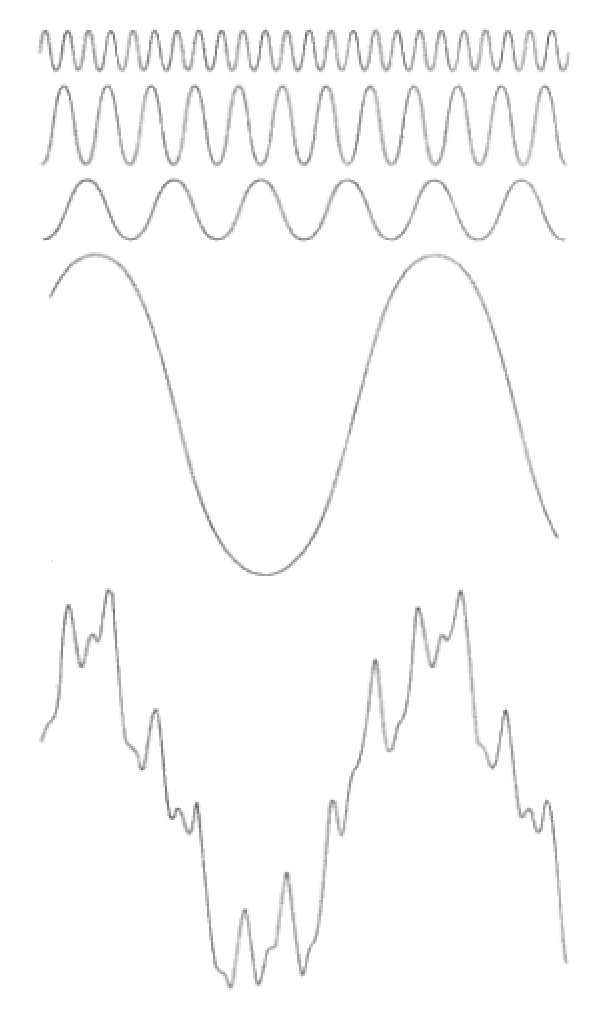
\includegraphics[scale=0.6]{pic1.png}
	\caption{底部函数是上面四个函数的和}
\end{figure}
由于我们在图像处理持续时间有限的函数(图像)。所以傅里叶变换使我们感兴趣的工具,接下来我将介绍一下傅里叶变换的一些性质以及他们在数字图像处理中的应用。
\section{基本概念\cite{.2010}}
\subsection{欧拉公式}
欧拉利用了i来表示$\sqrt{-1}$,并且得到了如下公式
\begin{equation}
	e^{i x}=\cos x+i \sin x
\end{equation}
并且由此可以推得:
\begin{equation}
	\cos x=\frac{e^{ix}+e^{-ix}}{2}, \sin x=\frac{e^{ix}-e^{-ix}}{2i}
\end{equation}
\subsection{傅里叶级数}
具有周期T的连续变量t的周期函数f(t)可以被描述成乘以适当系数的正弦项或余弦项和。我们知道,这就是傅里叶级数,他有如下性质:
\begin{equation}\label{3}
	f(t)=\sum_{n=-\infty}^{\infty} c_{n} \mathrm{e}^{\mathrm{j} \frac{2 \pi n}{T} t}
\end{equation}
其中,
\begin{equation}
	c_{n}=\frac{1}{T} \int_{-T / 2}^{T / 2} f(t) \mathrm{e}^{-\mathrm{j}^{\frac{2 \pi n}{T}}} \mathrm{d} t, \quad n=0,\pm 1,\pm 2, \cdots
\end{equation}
是系数。\eqref{3}展开为正弦项和余弦项之和这一事实来自欧拉公式。
\subsection{单位冲激}
连续变量t在t=0处的单位冲激表示为$\delta(t)$,其定义是
\begin{equation}
	\delta(t)=\left\{\begin{array}{ll}
		\infty, & t=0      \\
		0,      & t \neq 0
	\end{array}\right.\end{equation}
还被限制等式
\begin{equation}
	\int_{-\infty}^{\infty} \delta(t) \mathrm{d} t=1
\end{equation}
物理上,如果我们把t解释成时间,那么一个冲激就可以看成幅度无限、持续时间为0、具有单位面积的尖峰信号。
\subsection{连续变量函数的傅里叶变换}
由$\Im\{f(t)$表示的连续变量t的连续函数$f(t)$的傅里叶变换由下式定义:\footnote{傅里叶变换存在的充分条件是$f(t)$的绝对值或者平方的积分是有限的,实践中 傅里叶变换的存在性不是问题,但无限扩展的理想信号除外}
\begin{equation}
	\Im\{f(t)\}=\int_{-\infty}^{\infty} f(t) \mathrm{e}^{-\mathrm{j} 2 \pi \mu t} \mathrm{d} t
\end{equation}
其中,$\mu$也是一个连续变量。因为$t$被积分过了,所以$\Im\{f(t)\}$只是关于$\mu$的函数,为了明确这一事实,$f(t)$的傅里叶变换可以写成:
\begin{equation}
	f(\mu)=\int_{-\infty}^{\infty} f(t) \mathrm{e}^{-\mathrm{j} 2 \pi \mu t} \mathrm{d} t
\end{equation}
%\end{multicols}
相反,给定$F(\mu)$,通过傅里叶反变换k可以获得$f(t)$,即$f(t)=\Im^{-1}{F(\mu)}$,写为
\begin{equation}
	f(t)=\int_{-\infty}^{\infty} f(\mu) \mathrm{e}^{\mathrm{j} 2 \pi \mu t} \mathrm{d} \mu
\end{equation}
上面两式合起来被称为傅里叶变换对。他们指出了一个重要的事实,即一个函数可以由其变换和逆变换恢复。\par
用欧拉公式,我们可以得到
\begin{equation}
	F(\mu)=\int_{-\infty}^{\infty} f(t)[\cos (2 \pi \mu t)-\mathrm{j} \sin (2 \pi \mu t)] \mathrm{d} t
\end{equation}
我们可以看到,如果f(t)是实数那么其变换通常是复数。注意,傅里叶变换是$f(t)$乘以正弦项的展开,正弦项的频率由$\mu$的值来决定(如我们之前提到的,变量t被积分过了)。因为积分后做左边剩下的 唯一变量是频率,故我们说傅里叶变换域是频率域。其中频率  变量$\mu$的单位取决于$t$的单位。
\subsection{卷积}
两个函数的卷积涉及一个函数关于原点做翻转(旋转180度)并滑过另一个函数,在滑动过程中的每一个位移我们进行计算每个乘积的和。在这里我们感兴趣的是对于具有连续变量t的两个连续函数$f(t)$和$h(t)$的卷积因此我们用积分代替求和。卷积定义如下
\begin{equation}
	f(t) * h(t)=\int_{-\infty}^{\infty} f(\tau) h(t-\tau) \mathrm{d} \tau
\end{equation}
其中,负号代表之前的反转,t是一个函数滑过另一个函数的位移,而$\tau$是积分假变量。现在我们假设函数从$-\infty$扩展到$\infty$
\section{取样和取样函数的傅里叶变换\cite{Gonzalez.2009}}
\subsection{取样}
在计算机处理之前,连续函数必须转换为离散值序列。在下面讨论中我们将详细讨论取样。\par
考虑一个连续函数$f(t)$,我们希望以独立变量t的均匀间隔$\Delta T$取样。我们假定函数从$-\infty$扩展到$\infty$,模拟取样的一种方法是用一个单位间隔$\Delta T$的冲激串作为取样函数去乘以$f(t)$,即
\begin{equation}\tilde{f}(t)=f(t) s_{\Delta T}(t)=\sum_{n=-\infty}^{\infty} f(t) \delta(t-n \Delta T)\end{equation}
其中$\tilde{f}(t)$表示取样后的函数。这一和式的每一个分量都是由在该冲激位置$f(t)$的值加权后的冲激。每个取样值由加权后的冲激“强度”给出,我们可以通过积分得到它。也就是序列中的任意取样值$f_{k}$由下式给出
\begin{equation}
	f_{k}=\int_{-\infty}^{\infty}f(t)\delta(t-k\Delta T)\mathrm{d}t=f(k\Delta T)
\end{equation}
图2是原始函数均匀采样的结果
\begin{figure}[ht]
	\centering
	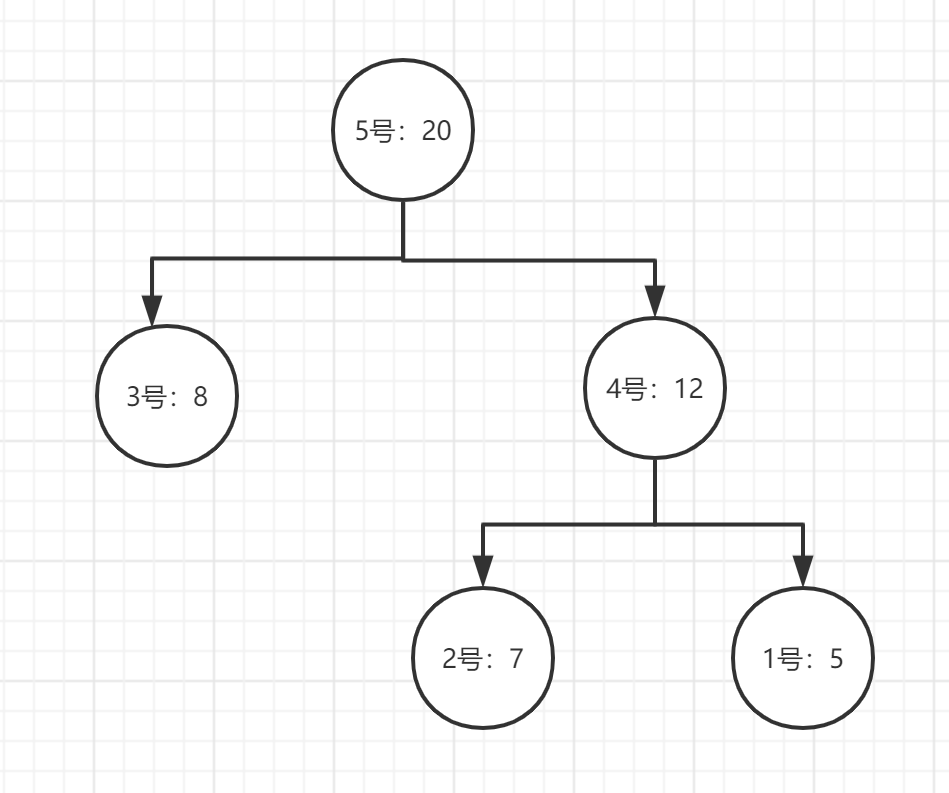
\includegraphics[scale=0.6]{pic2.png}
	\caption{对于连续函数进行采样}
\end{figure}
\subsection{取样函数的傅里叶变换}
令$F(\mu)$代表连续函数$f(t)$的傅里叶变换,取样后的相应变换$\tilde{f}(t)$是$f(t)$与一个冲激串的乘积。由卷积定理可知,空间域两个函数的傅里叶变换是两个函数在频率域的卷积,这样取样后的函数$\tilde{f}(t)$的傅里叶变换$\tilde{F}(\mu)$是
\begin{equation}\tilde{F}(\mu)=\Im\{\tilde{f}(t)\}=\Im\left\{f(t) s_{\Delta T}(t)\right\}=F(\mu) \star S(\mu)\end{equation}
其中由冲激串的傅里叶变换可得
\begin{equation}S(\mu)=\frac{1}{\Delta T} \sum_{n=-\infty}^{\infty} \delta\left(\mu-\frac{n}{\Delta T}\right)\end{equation}
由定义我们可以直接得到$F(\mu)$$S(\mu)$的卷积:
	\begin{equation}\begin{aligned}
			\tilde{F}(\mu) & =F(\mu) \star S(\mu)=\int_{-\infty}^{\infty} F(\tau) S(\mu-\tau) \mathrm{d} \tau                                                                                                                                                                                                         \\
			               & =\frac{1}{\Delta T} \int_{-\infty}^{\infty} F(\tau) \sum_{n=-\infty}^{\infty} \delta\left(\mu-\tau-\frac{n}{\Delta T}\right) \mathrm{d} \tau=\frac{1}{\Delta T} \sum_{n=-\infty}^{\infty} \int_{-\infty}^{\infty} F(\tau) \delta\left(\mu-\tau-\frac{n}{\Delta T}\right) \mathrm{d} \tau \\
			               & =\frac{1}{\Delta T} \sum_{n=-\infty}^{\infty} F\left(\mu-\frac{n}{\Delta T}\right)
		\end{aligned}\end{equation}
	其中最后一步来自于冲激取样的特性。\par
	显然,虽然$\tilde{f}(t)$是取样后的函数,但其变换$\tilde{F}(\mu)$是连续的。
	\section{由取样后的数据重建(复原)函数\cite{Gonzalez.2009}}
	\subsection{取样函数的逆傅里叶变换}
	用一组样本集合来重建函数实际上可以减少样本内插。即使简单的用显示介质显示一组图像的行为都要求来自其样本的图像重建。因此理解取样数据重建是很重要的。卷积是这一理解的核心。\par
	使用卷积定理我们可以知道,
	\begin{equation}f(t)=\delta^{-1}\{F(\mu)\}=\delta^{-1}\{H(\mu) \tilde{F}(\mu)\}=h(t) * \tilde{f}(t)\end{equation}
	不加证明的,可以得到$f(t)$的如下空间域表达式:
	\begin{equation}f(t)=\sum_{n=-\infty}^{\infty} f(n \Delta T) \operatorname{sinc}[(t-n \Delta T) / \Delta T]\end{equation}
	其中,$sinc$函数定义为$\operatorname{sinc}(m)=\frac{\sin (\pi m)}{(\pi m)}$\par
	上式表明重建的函数是用取样值加权的sinc函数的无限和,并且由重要的特性,即重建的函数恒等于多个$\Delta T$的整数增量处的样本值。
\section{图像处理进行傅里叶变换的意义}
其实量化这个概念在我这个学期做单片机大作业的时候有涉及,在表示音乐的音调的时候,需要将不同的音调转化不同的频率。但因为音调在乐谱中不是一个连续的概念(完成品类似于八音盒),所以没有用到傅里叶变换,而是用到了其他的公式。不过对于图像来说,如果看作是一个频率域滤波,那么就是一个连续的概念了。
傅里叶变换的意义就是给出了一个在频域解决问题的方法,虽然当时没有什么物理上的证明,不过到了现代,我们知道傅里叶是对的了。首先,复杂一点的波,比如声波确实是更简单的多个不同正弦波组成的。利用这点,我们可以有效进行数字降噪,比如一段音频文件,混入了汽车发动机的声音,说话声变的难以听到。我们对这段音频文件的声波波形做傅里叶变换,可以等到一个展开式,然后找出发动机噪声的频率,可以做到去噪声。\par
傅立叶变换在实际中有非常明显的物理意义,设f是一个能量有限的模拟信号,则其傅立叶变换就表示f的谱。从纯粹的数学意义上看,傅立叶变换是将一个函数转换为一系列周期函数来处理的。从物理效果看,傅立叶变换是将图像从空间域转换到频率域,其逆变换是将图像从频率域转换到空间域。换句话说,傅立叶变换的物理意义是将图像的灰度分布函数变换为图像的频率分布函数,傅立叶逆变换是将图像的频率分布函数变换为灰度分布函数。

\section{结语}
因为时间和储备知识的限制,所以在本文只讨论了傅里叶变换的基本原理以及它与数字图像处理(频率域滤波)之间的关系。上面只
是一个对于我能看懂的知识进行一个阐述。因为平时实验室做的课题主要偏向于
神经网络对于图像处理的应用,对于基础的数字图像处理方法是从零开始的。这次的论文仅作为我对传统数字图像处理的初次
探讨。
% \begin{thebibliography}{1}

% 	\bibitem{1}
% 	冈萨雷斯.数字图像处理(第三版)

% 	\bibitem{2}
% 	四川大学数学教研室.高等数学(第四册第三版)

% \end{thebibliography}
\bibliographystyle{ieeetr}
\bibliography{ref}
\end{document}